\documentclass[12pt, a4paper]{article}

% Package Includes
% Blindtext verwenden
\usepackage{blindtext}

% IF statements verwenden
\usepackage{ifthen}

% Texte einfärben
\usepackage{color}
\definecolor{orange}{rgb}{1,0.5,0}

% Code Snippets einfügen
\usepackage{listings}

% Code Formatting für JavaScript
\lstdefinelanguage{JavaScript}{
  keywords={break, case, catch, continue, debugger, default, delete, do, else, finally, for, function, if, in, instanceof, new, return, switch, this, throw, try, typeof, var, void, while, with},
  keywordstyle=\color{blue}\bfseries,
  ndkeywords={class, export, boolean, throw, implements, import, this},
  ndkeywordstyle=\color{darkgray}\bfseries,
  identifierstyle=\color{black},
  sensitive=false,
  comment=[l]{//},
  morecomment=[s]{/*}{*/},
  commentstyle=\color{purple}\ttfamily,
  stringstyle=\color{orange}\ttfamily,
  morestring=[b]',
  morestring=[b]"
}

\lstset{
  backgroundcolor=\color{white},
  frame=single,
  keywordstyle=\color{blue},
  numbers=left,
  language=bash,
  breaklines=true}

% weitere Pakete
% Grafiken aus PNG Dateien einbinden
\usepackage{graphicx}
\graphicspath{ {00_Assets/00_Images/} }

% deutsche Silbentrennung
\usepackage[ngerman]{babel}

% Eurozeichen einbinden
\usepackage[right]{eurosym}

% Umlaute unter UTF8 nutzen
\usepackage[utf8]{inputenc}

% Zeichenencoding
\usepackage[T1]{fontenc}
\usepackage{lmodern}
\usepackage{fix-cm}

% keine Silbentrennung
\usepackage[none]{hyphenat}
\sloppy

% Tabellen
\usepackage{tabularx}
\usepackage{floatrow}
\floatsetup[table]{capposition=top}

% Mathematische Symbole importieren
\usepackage{amssymb}

% Zitieren
\usepackage{cite}
% Festlegung Art der Zitierung
\bibliographystyle{ieeetr}

% Paket für Zeilenabstand
\usepackage[onehalfspacing]{setspace}

% Paket für multicol Umgebung
\usepackage{multicol}

% für Stichwortverzeichnis
\usepackage{makeidx}

% für Abkürzungsverzeichnis
\usepackage[nohyperlinks, printonlyused, withpage, smaller]{acronym}

% Indexerstellung
\makeindex

% Package für Anhänge
\usepackage[toc,page]{appendix}

% Package für Fußtnoten
\usepackage[hang]{footmisc}
\setlength{\footnotemargin}{1em}
\setlength{\skip\footins}{3em}

% Auf jeder Seite Überschrift anzeigen
%\pagestyle{headings}

% Package für Abkürzungsverzeichnis
% --- Abkürzungsverzeichnis: ----------------------------
\usepackage[german]{nomencl}
% Befehl umbenennen in abk
\let\abk\nomenclature
% Deutsche Überschrift
\renewcommand{\nomname}{Abkürzungsverzeichnis}
% Punkte zw. Abkürzung und Erklärung
\setlength{\nomlabelwidth}{.40\hsize}
\renewcommand{\nomlabel}[1]{#1 \dotfill}
% Zeilenabstände verkleinern
\setlength{\nomitemsep}{-\parsep}
\makenomenclature
%--------------------------------------------------------

% Seitenränder einstellen
\usepackage[left=30mm, right=30mm, top=35mm, bottom=35mm]{geometry}


% Variablen
\newcommand{\firma}{<Company>}
\newcommand{\titel}{<Document Title>}
\newcommand{\autor}{<Author>}
\newcommand{\id}{<ID>}
\newcommand{\arbeitstyp}{<Document Type>}
\newcommand{\arbeitstypeartikel}{<Article>}
\newcommand{\fach}{<Lecture (optional)>}
\newcommand{\betreuertitel}{<Title>}
\newcommand{\betreuer}{<Name>}
\newcommand{\abgabedatum}{<Date>}
\newcommand{\subject}{<Subject>}
\newcommand{\keywords}{<Keyword1>, <Keyword2>}


% Toggles
% show / hide Sperrvermerk
\newboolean{showSperrvermerk}
\setboolean{showSperrvermerk}{true}

% show / hide Eidesstaatliche Erklärung
\newboolean{showErklaerung}
\setboolean{showErklaerung}{true}

% show / hide list of figures
\newboolean{showListOfFigures}
\setboolean{showListOfFigures}{true}

% show / hide list of tables
\newboolean{showListOfTables}
\setboolean{showListOfTables}{true}

% show / hide listings
\newboolean{showListings}
\setboolean{showListings}{true}

% show / hide abbreviations
\newboolean{showAbbr}
\setboolean{showAbbr}{true}

% Hyperlinks in PDF Datei
\usepackage[colorlinks,
pdfpagelabels,
pdfstartview = FitH,
bookmarksopen = true,
bookmarksnumbered = true,
linkcolor = black,
plainpages = false,
hypertexnames = false,
citecolor = black,
hidelinks,
pdftitle={\titel},
pdfsubject={\subject},
pdfauthor={\autor},
pdfkeywords={\keywords}
] {hyperref}

% Dokumenten Beginn
\begin{document}

% Titelseite
\begin{titlepage}
    \ifthenelse{\boolean{customTitlepage}}{
        \centering
{\scshape\LARGE \firma \par}
\vspace{1cm}
{\scshape\Large \arbeitstyp \par}
\vspace{1.5cm}
{\line(1,0){400} \par}
{\huge\bfseries \titel \par}
{\line(1,0){400} \par}
\vspace{2cm}
{\Large \fach \par }
\vspace{1cm}
{\Large\itshape \autor \par}
{\itshape \id \par}
\vfill
{betreut durch \par}
{\betreuertitel \ \betreuer \par}
\vfill
{\large \abgabedatum \par}

    }{
    \centering
        {\scshape\LARGE \firma \par}
        \vspace{1cm}
        {\scshape\Large \arbeitstyp \par}
        \vspace{1.5cm}
        {\line(1,0){400} \par}
        {\huge\bfseries \titel \par}
        {\line(1,0){400} \par}
        \vspace{2cm}
        {\Large \fach \par }
        \vspace{1cm}
        {\Large\itshape \autor \par}
        {\itshape \id \par}
        \vfill
        {betreut durch \par}
        {\betreuertitel \ \betreuer \par}
        \vfill
        {\large \abgabedatum \par}
    }
\end{titlepage}

\newpage
\pagenumbering{Roman}

\setcounter{page}{2}

% Abstract einbinden
\section*{Abstract}
Lorem ipsum dolor sit amet, consetetur sadipscing elitr, sed diam nonumy eirmod tempor invidunt ut labore et dolore magna aliquyam erat, sed diam voluptua. At vero eos et accusam et justo duo dolores et ea rebum. Stet clita kasd gubergren, no sea takimata sanctus est Lorem ipsum dolor sit amet. Lorem ipsum dolor sit amet, consetetur sadipscing elitr, sed diam nonumy eirmod tempor invidunt ut labore et dolore magna aliquyam erat, sed diam voluptua. At vero eos et accusam et justo duo dolores et ea rebum. Stet clita kasd gubergren, no sea takimata sanctus est Lorem ipsum dolor sit amet. Lorem ipsum dolor sit amet, consetetur sadipscing elitr, sed diam nonumy eirmod tempor invidunt ut labore et dolore magna aliquyam erat, sed diam voluptua. At vero eos et accusam et justo duo dolores et ea rebum. Stet clita kasd gubergren, no sea takimata sanctus est Lorem ipsum dolor sit amet.   

\begin{figure}[h]
  \centering
  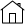
\includegraphics{00_Data/01_Assets/00_Images/test}
  \caption{Test Bild von einem Haus}
  \label{img:haus}
\end{figure}

\newpage

% Inhaltsverzeichnis anzeigen
\tableofcontents

\newpage

% Sperrvermerk
\ifthenelse{\boolean{showSperrvermerk}}{
  \addcontentsline{toc}{section}{Sperrvermerk}
  \section*{Sperrvermerk}
  \arbeitstypeartikel \ vorliegende \arbeitstyp \ beinhaltet vertrauliche Informationen der \firma. Veröffentlichung und Vervielfältigung ist ohne vorherige schriftliche Genehmigung der \firma \ nicht gestattet. \arbeitstypeartikel \ \arbeitstyp \ ist nur den Gutachtern und den Mitgliedern des Prüfungsausschusses zugänglich zu machen.
  \\\\\\\\
  \vspace{5cm}
  \begin{tabularx}{\textwidth}[b]{p{5cm} X p{5cm}} \cline{1-1} \cline{3-3}
  Datum & & \betreuer
  \end{tabularx}
  \newpage
}

% Eidesstaatliche Erklärung
\ifthenelse{\boolean{showErklaerung}}{
  \addcontentsline{toc}{section}{Eidesstaatliche Erklärung}
  \section*{Eidesstaatliche Erklärung}
  Hiermit versichere ich, dass ich die vorliegende Arbeit selbstständig und ohne Benutzung anderer als der angegebenen Hilfsmittel angefertigt habe. Alle Stellen, die wörtlich oder sinngemäß aus anderen Schriften entnommen wurden, sind als solche kenntlich gemacht.
  \\\\
  Die Arbeit ist noch nicht veröffentlicht oder anderweitig für Prüfungszwecke vorgelegt worden.
  \\\\\\\\
  \vspace{5cm}
  \begin{tabularx}{\textwidth}[b]{p{5cm} X p{5cm}} \cline{1-1} \cline{3-3}
  Datum & & \autor
  \end{tabularx}
}

\newpage

% Abbildungsverzeichnis
\ifthenelse{\boolean{showListOfFigures}}{
  \addcontentsline{toc}{section}{Abbildungsverzeichnis}
  \listoffigures
}

\newpage

% Tabellenverzeichnis
\ifthenelse{\boolean{showListOfTables}}{
  \addcontentsline{toc}{section}{Tabellenverzeichnis}
  \listoftables
}

\newpage

% Abkürzungsverzeichnis
\ifthenelse{\boolean{showAbbr}}{
  \addcontentsline{toc}{section}{Abkürzungsverzeichnis}
  \printnomenclature
}

\newpage

% Listings
\ifthenelse{\boolean{showListings}}{
  \addcontentsline{toc}{section}{Listings}
  \lstlistoflistings
}

\newpage

% Beginn der Seitenzählung
\setcounter{page}{1}
\pagenumbering{arabic}

% Hier werden die einzelnen Kapitel eingelesen
\IfFileExists{./00_Data/00_Chapters/chapter1}{\section{Einführung}
\subsection{Themenstellung}
Lorem ipsum dolor sit amet, consetetur sadipscing elitr, sed diam nonumy eirmod tempor invidunt ut labore et dolore magna aliquyam erat, sed diam voluptua. At vero eos et accusam et justo duo dolores et ea rebum. Stet clita kasd gubergren, no sea takimata sanctus est Lorem ipsum dolor sit amet. Lorem ipsum dolor sit amet, consetetur sadipscing elitr, sed diam nonumy eirmod tempor invidunt ut labore et dolore magna aliquyam erat, sed diam voluptua. At vero eos et accusam et justo duo dolores et ea rebum. Stet clita kasd gubergren, no sea takimata sanctus est Lorem ipsum dolor sit amet. Lorem ipsum dolor sit amet, consetetur sadipscing elitr, sed diam nonumy eirmod tempor invidunt ut labore et dolore magna aliquyam erat, sed diam voluptua. At vero eos et accusam et justo duo dolores et ea rebum. Stet clita kasd gubergren, no sea takimata sanctus est Lorem ipsum dolor sit amet.   
\subsection{Vorgehensweise}
Lorem ipsum dolor sit amet, consetetur sadipscing elitr, sed diam nonumy eirmod tempor invidunt ut labore et dolore magna aliquyam erat, sed diam voluptua. At vero eos et accusam et justo duo dolores et ea rebum. Stet clita kasd gubergren, no sea takimata sanctus est Lorem ipsum dolor sit amet. Lorem ipsum dolor sit amet, consetetur sadipscing elitr, sed diam nonumy eirmod tempor invidunt ut labore et dolore magna aliquyam erat, sed diam voluptua. At vero eos et accusam et justo duo dolores et ea rebum. Stet clita kasd gubergren, no sea takimata sanctus est Lorem ipsum dolor sit amet. Lorem ipsum dolor sit amet, consetetur sadipscing elitr, sed diam nonumy eirmod tempor invidunt ut labore et dolore magna aliquyam erat, sed diam voluptua. At vero eos et accusam et justo duo dolores et ea rebum. Stet clita kasd gubergren, no sea takimata sanctus est Lorem ipsum dolor sit amet.   
\subsection{Zielsetzung}
Lorem ipsum dolor sit amet, consetetur sadipscing elitr, sed diam nonumy eirmod tempor invidunt ut labore et dolore magna aliquyam erat, sed diam voluptua. At vero eos et accusam et justo duo dolores et ea rebum. Stet clita kasd gubergren, no sea takimata sanctus est Lorem ipsum dolor sit amet. Lorem ipsum dolor sit amet, consetetur sadipscing elitr, sed diam nonumy eirmod tempor invidunt ut labore et dolore magna aliquyam erat, sed diam voluptua. At vero eos et accusam et justo duo dolores et ea rebum. Stet clita kasd gubergren, no sea takimata sanctus est Lorem ipsum dolor sit amet. Lorem ipsum dolor sit amet, consetetur sadipscing elitr, sed diam nonumy eirmod tempor invidunt ut labore et dolore magna aliquyam erat, sed diam voluptua. At vero eos et accusam et justo duo dolores et ea rebum. Stet clita kasd gubergren, no sea takimata sanctus est Lorem ipsum dolor sit amet.   
\subsection{Stand der Technik}
Lorem ipsum dolor sit amet, consetetur sadipscing elitr, sed diam nonumy eirmod tempor invidunt ut labore et dolore magna aliquyam erat, sed diam voluptua. At vero eos et accusam et justo duo dolores et ea rebum. Stet clita kasd gubergren, no sea takimata sanctus est Lorem ipsum dolor sit amet. Lorem ipsum dolor sit amet, consetetur sadipscing elitr, sed diam nonumy eirmod tempor invidunt ut labore et dolore magna aliquyam erat, sed diam voluptua. At vero eos et accusam et justo duo dolores et ea rebum. Stet clita kasd gubergren, no sea takimata sanctus est Lorem ipsum dolor sit amet. Lorem ipsum dolor sit amet, consetetur sadipscing elitr, sed diam nonumy eirmod tempor invidunt ut labore et dolore magna aliquyam erat, sed diam voluptua. At vero eos et accusam et justo duo dolores et ea rebum. Stet clita kasd gubergren, no sea takimata sanctus est Lorem ipsum dolor sit amet.   }{}
\IfFileExists{./00_Data/00_Chapters/chapter2}{\section{Grundlagen}
\subsection{Einführung}
\subsection{Begriffserklärungen}}{}
\IfFileExists{./00_Data/00_Chapters/chapter3}{\section{Chapter 3}}{}
\IfFileExists{./00_Data/00_Chapters/chapter4}{\section{Chapter 4}}{}
\IfFileExists{./00_Data/00_Chapters/chapter5}{\section{Chapter 5}}{}
\IfFileExists{./00_Data/00_Chapters/chapter6}{\include{00_Data/00_Chapters/chapter6}}{}

\newpage
\pagenumbering{roman}
\setcounter{page}{10}

% Literatur
\addcontentsline{toc}{section}{Literatur}
\bibliography{00_Data/02_Bib/mybib}

\newpage

% Anhänge
% Appendix
\newpage
\begin{appendix}
  \section{Test Appendix}\label{app:test}
\end{appendix}

\end{document}
